\documentclass[]{article}
\newcommand{\FileDepth}{../../..}
\usepackage[letterpaper, landscape, margin=0.5cm]{geometry}
\usepackage[T1]{fontenc}
\usepackage{textcomp}%Not strictly necessary, but gives \textmu command for "micro."
\usepackage{fancyhdr}
\usepackage{amsmath}
\usepackage{amssymb}
\usepackage{graphicx}
\usepackage{xcolor}
\usepackage{tikz}
\usetikzlibrary{calc}
\usepackage[shortlabels]{enumitem}
\usepackage{multicol}
\usepackage{vwcol}
\usepackage{hyperref}
\usepackage{wrapfig}
%opening
\newcommand{\SecType}{L}
\newcommand{\Week}{13}
\title{PH 211 Lecture \Week}
\author{Benjamin Bauml}
\date{Summer 2024}

\newcommand{\Purpose}{4}
\newcommand{\DefOnly}{0}

\input{\FileDepth/Formats/Assignment20240614.tex}
\usepackage[absolute]{textpos}
% This package relies on Assignment Format 2024-06-14 or later to work. It is recommended that the Purpose and DefOnly commands be given as such:
%\newcommand{\Purpose}{4}
%\newcommand{\DefOnly}{0}
% Activities need to be entered outside of the TeacherMargin and PresentSpace environments, otherwise they will be defined only locally. They can even go in the preamble.
\newenvironment{TeacherMargin}{\begin{textblock*}{10.8cm}(0.5cm,0.5cm)
\small}{\end{textblock*}
\hspace{0.1cm}}
\newenvironment{PresentSpace}{\begin{textblock*}{0.3cm}(26.85cm,9.35cm)
--
\end{textblock*}
\begin{textblock*}{15.6cm}(11.8cm,0.5cm)
\begin{Repurpose}{1}
\Large}{\end{Repurpose}
\end{textblock*}
\hspace{0.1cm}}

\newcommand{\FBDaxes}[4][2]{
	\begin{scope}[shift={(#2)},rotate=#3]
		% x-axis
		\draw[thick,->] (-#1,0) -- (#1,0);
		\node[anchor=west] at (#1,0) {$x$};
		% y-axis
		\draw[thick,->] (0,-#1) -- (0,#1);
		\node[anchor=south] at (0,#1) {$y$};
		\coordinate (#4) at (0,0);
	\end{scope}
}
\newcommand{\FBDvectorMA}[4]{
	\begin{scope}[shift={(#1)}]
		\coordinate (#4tip) at ({#2*cos(#3)},{#2*sin(#3)});
		\draw[ultra thick,blue,->] (#1) -- (#4tip);
	\end{scope}
}
\newcommand{\FBDvectorXY}[3]{
	\begin{scope}[shift={(#1)}]
		\coordinate (#3tip) at (#2);
		\draw[ultra thick,blue,->] (0,0) -- (#3tip);
	\end{scope}
}
\newcommand{\FBDdot}[1]{
	\filldraw[black] (#1) circle (3pt);
}
\newcommand{\FBDbox}[5][1]{
	\begin{scope}[shift={(#2)},rotate=#3]
		\filldraw[color=black,fill=white,thick] ({-#1/2},{#1/2}) -- ({-#1/2},{-#1/2}) -- ({#1/2},{-#1/2}) -- ({#1/2},{#1/2}) -- cycle;
		% Left side coordinates
		\coordinate (#4ltq) at ({-#1/2},{#1/4});
		\coordinate (#4lcent) at ({-#1/2},0);
		\coordinate (#4lbq) at ({-#1/2},{-#1/4});
		% right side coordinates
		\coordinate (#4rtq) at ({#1/2},{#1/4});
		\coordinate (#4rcent) at ({#1/2},0);
		\coordinate (#4rbq) at ({#1/2},{-#1/4});
		% top coordinates
		\coordinate (#4tlq) at ({-#1/4},{#1/2});
		\coordinate (#4tcent) at (0,{#1/2});
		\coordinate (#4trq) at ({#1/4},{#1/2});
		% bottom coordinates
		\coordinate (#4blq) at ({-#1/4},{-#1/2});
		\coordinate (#4bcent) at (0,{-#1/2});
		\coordinate (#4brq) at ({#1/4},{-#1/2});
		% corners
		\coordinate (#4tl) at ({-#1/2},{#1/2});
		\coordinate (#4tr) at ({#1/2},{#1/2});
		\coordinate (#4bl) at ({-#1/2},{-#1/2});
		\coordinate (#4br) at ({#1/2},{-#1/2});
		\node at (0,0) {#5};
	\end{scope}
}
%\newcommand{\MVec}[3][0]{%Creates a momentum vector of length #3 centered at #2 and rotated #1 degrees counterclockwise.
	\begin{scope}[rotate=#1,shift={(#2)}]
		\draw[->,thick] ({-#3/2},0) -- ({#3/2},0);
	\end{scope}
}
\newcommand{\MDot}[1]{%Creates a dot at #1 to represent a zero vector.
	\filldraw (#1) circle (1pt);
}
\newcommand{\MVDRows}[2][4.5]{%Creates the rows (initial, delta, final) of a momentum vector diagram. The optional argument determines the width of the table, and defaults to a good length for three columns (two objects and the total system). The non-optional argument gives a coordinate name (not displayed) to the diagram.
	\begin{scope}
		%\draw[thick] (0,5.5) -- (0,0);
		\draw[thick] (-1,4.5) -- (#1,4.5);
		\node at (-0.5,3.75) {$\vec{p}_{i}$};
		\draw[thick] (-1,3) -- (#1,3);
		\node at (-0.5,2.25) {$\Delta\vec{p}$};
		\draw[thick] (-1,1.5) -- (#1,1.5);
		\node at (-0.5,0.75) {$\vec{p}_{f}$};
		\coordinate (#2) at (0,5);
	\end{scope}
}
\newcommand{\MVDCol}[4][0.75]{%Creates a column for an object in a momentum vector diagram. The first (non-optional) argument is the coordinate name (not displayed) of the column, while the second is the displayed column header. The first argument also names the three entries down the column. The third argument anchors the column, so it should either be the coordinate name of the MVD (for the first column) or the coordinate name of the previous column. The optional argument indicates how far the center of the column should be from the previous column's edge, and defaults to 0.75.
	\begin{scope}[shift={(#4)}]
		\node at (#1,0) {#3};
		%\draw[thick] ({#1*2},0.5) -- ({#1*2},-5);
		\draw[thick] (0,0.5) -- (0,-5);
		\coordinate (#2init) at (#1,-1.25);
		\coordinate (#2delt) at (#1,-2.75);
		\coordinate (#2fin) at (#1,-4.25);
		\coordinate (#2) at ({#1*2},0);
	\end{scope}
}

%\input{\FileDepth/Activities/Activity_One/Activity_One.tex}
%\input{\FileDepth/Activities/Activity_Two/Activity_Two.tex}

\begin{document}
\begin{TeacherMargin}

\end{TeacherMargin}
\begin{PresentSpace}
\begin{center}
	\huge Lecture \Week: Newton' 3rd Law of Motion \\
	\small (and a Bit of Springs)
\end{center}
\vspace{0.5cm}
\underline{Warm-Up Activity} \\
Which of the following statements, if any, are true about Newton's 3rd law pairs?
\begin{enumerate}[(A)]
	\item They appear on different free-body diagrams.
	\item They are the same type of force.
	\item They appear on the same free-body diagram.
	\item $\vec{F}^{t}_{AB} = -\vec{F}^{t}_{AB}$
\end{enumerate}
\vspace{1cm}
\underline{Feedback Question} \\
Do you prefer feedback through documents uploaded to Canvas, or through Gradescope (as was done on the quizzes)?
%\begin{multicols}{2}
\begin{enumerate}[(A)]
	\item PDFs on Canvas
	\item Comments in Gradescope
\end{enumerate}
%\end{multicols}
\end{PresentSpace}
\newpage
\begin{TeacherMargin}

\end{TeacherMargin}
\begin{PresentSpace}
\vspace{-10pt}
\section*{Newton's 3rd Law of Motion}
\vspace{-10pt}
\begin{itemize}
	\item If A exerts a force on B, then B exerts a force of the same magnitude on A in the opposite direction:
	\[
	\vec{F}^{t}_{AB} = -\vec{F}^{t}_{BA}
	\]
	\item These two forces make a \textit{Newton's 3rd law pair}, or an \textit{action-reaction pair}.
	\item 3rd law pair forces\dots
	\begin{itemize}
		\item are the same type of force;
		\item appear on different free body diagrams.
	\end{itemize}
\end{itemize}
\end{PresentSpace}
\newpage
\begin{TeacherMargin}
\noindent\textbf{The Negative Sign} \\
The negative sign tells us that the force of the spring points opposite the displacement from equilibrium. The spring wants to return to its \\
unstretched/uncompressed length. Forces that try to return a system to equilibrium are called \textit{restoring forces}.
\end{TeacherMargin}
\begin{PresentSpace}
\vspace{-10pt}
\section*{Spring Forces}
\vspace{-10pt}
\begin{itemize}
	\item Many objects resist changes in physical configuration (\textit{i.e.} deformations).
	\item For small deformations, we can model the object as a spring.
	\item The forces caused by springs obey Hooke's law: $\vec{F}^{S} = -k(\vec{x}-\vec{x}_{eq})$.
	\begin{itemize}
		\item $\Delta\vec{x} = (\vec{x}-\vec{x}_{eq})$ is displacement from equilibrium.
		\item $k$ is the spring constant.
		\item What does the negative sign mean?
	\end{itemize}
\end{itemize}
\end{PresentSpace}
\newpage
\begin{TeacherMargin}

\end{TeacherMargin}
\begin{PresentSpace}
\vspace{-10pt}
\section*{Types of Forces}
\vspace{-10pt}
\begin{itemize}
	\item Gravity \qquad \qquad \qquad \qquad $\vec{F}^{g}_{AB} = m_{A}\vec{g}_{B}$
	\begin{itemize}
		\item Newtonian \qquad\ $\vec{g}_{B} = G\frac{M_{B}}{r^{2}}(-\hat{r})$, $G = 6.67408\times10^{-11}\text{ N}\cdot\text{m}^{2}/\text{kg}^{2}$
		\item Near-Earth \qquad $\vec{g}_{E} = g(-\hat{y}),\ g=9.81\frac{\text{m}}{\text{s}^{2}} \approx 10\frac{\text{m}}{\text{s}^{2}}$
	\end{itemize}
	\item Normal \qquad $\vec{F}^{N}$ always $\bot$; varies in magnitude
	\item Tension \qquad $\vec{F}^{T}$ uniform (massless, inextensible rope)
	\item Spring \qquad $\vec{F}^{S}=-k(\vec{x}-\vec{x}_{eq})$
	\item Friction
	\begin{itemize}
		\item Static Friction \qquad $F^{sf}\leq\mu_{s}|\vec{F}^{N}|$
		\item Kinetic Friction \qquad $F^{kf}=\mu_{k}|\vec{F}^{N}|$
	\end{itemize}
\end{itemize}
\end{PresentSpace}
\begin{textblock*}{5cm}(22cm,6cm)
	\Large
	\noindent\textbf{Not Forces}
	\begin{itemize}
		\normalsize
		\item Momentum
		\item Inertia
		\item Velocity
		\item Acceleration
	\end{itemize}
\end{textblock*}
\newpage
\begin{TeacherMargin}

\end{TeacherMargin}
\begin{PresentSpace}
\vspace{-10pt}
\section*{A*R*C*S: Uh-Oh Dr. Paws}
%\vspace{-10pt}
In the video in Section 3.16 of our textbook, Paul pushes a footstool (mass $m_{1}$) across the floor with a constant force so that the footstool speeds up. Dr. Paws (a dog with mass $m_{2}$) is sitting on the footstool. The coefficient of static friction between the dog and the footstool is $\mu$ (assume no friction between the footstool and the ground). How much force can Paul exert on the footstool before the dog begins sliding?
\end{PresentSpace}
\newpage
\begin{TeacherMargin}

\end{TeacherMargin}
\begin{PresentSpace}
\vspace{-10pt}
\section*{L\Week-1: Uh-Oh Dr. Paws -- Analyze and Represent}
\vspace{-10pt}
\begin{multicols}{2}
	\textbf{(1a) Understand the Problem}
	\begin{itemize}
		\large
		\item Mass of the footstool: $m_{1}=10\text{ kg}$
		\item Mass of the dog: $m_{2}=30\text{ kg}$
		\item Gravity: $g=10\text{ m/s}^{2}$
		\item Coefficient of static friction: $\mu=0.4$
	\end{itemize}
	\textbf{(1b) Identify Assumptions}
	\begin{itemize}
		\large
		\item Near-Earth
		\item Particle model
		\item Neglect air-resistance
		\item Dr. Paws doesn't move.
	\end{itemize}
	\textbf{(1c) Represent Physically}
	\begin{center}
		\begin{tikzpicture}
			\FBDaxes{0,0}{0}{dogaxes}
			\FBDaxes{3,-2}{0}{stoolaxes}
		\end{tikzpicture}
	\end{center}
\end{multicols}
\end{PresentSpace}
\newpage
\begin{TeacherMargin}

\end{TeacherMargin}
\begin{PresentSpace}
\vspace{-10pt}
\section*{L\Week-2: Uh-Oh Dr. Paws -- Sensemake}
\vspace{-10pt}

\end{PresentSpace}
\newpage
\begin{TeacherMargin}

\end{TeacherMargin}
\begin{PresentSpace}
\vspace{-10pt}
\section*{L\Week-3: Uh-Oh Dr. Paws -- Calculate}
\vspace{-10pt}

\end{PresentSpace}
\newpage
\begin{TeacherMargin}

\end{TeacherMargin}
\begin{PresentSpace}
\vspace{-10pt}
\section*{A Model for Interactions}
\vspace{-10pt}
\begin{itemize}
	\item Quantities
	\begin{itemize}
		\item Mass \quad $m$ \qquad \textbf{--} Force \quad $\vec{F}$
		%\item Force \quad $\vec{F}$
	\end{itemize}
	\item Laws
	\begin{itemize}
		\item Net force is proportional to acceleration: \\
		$\vec{F}^{net}=m\vec{a}$
		\item Forces come in pairs: $\vec{F}_{AB} = -\vec{F}_{BA}$
	\end{itemize}
	\item Asssumptions
	\begin{itemize}
		\item We can treat multiple objects as a system.
		\item All forces act as if on the center of the system.
	\end{itemize}
\end{itemize}
\end{PresentSpace}
\begin{textblock*}{5cm}(22cm,1.34cm)
\Large
\begin{itemize}
	\item Diagram
\end{itemize}
\centering
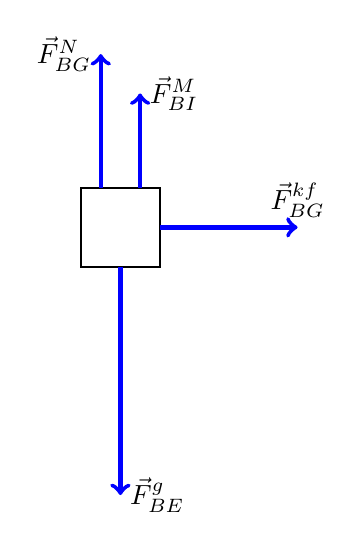
\begin{tikzpicture}
	\FBDbox{0,0}{0}{box}{}
	\FBDvectorXY{boxtrq}{0,1.2}{FM}
	\node[anchor=west] at (FMtip) {$\vec{F}^{M}_{BI}$};
	\FBDvectorXY{boxtlq}{0,1.7}{FN}
	\node[anchor=east] at (FNtip) {$\vec{F}^{N}_{BG}$};
	\FBDvectorXY{boxrcent}{1.75,0}{FKF}
	\node[anchor=south] at (FKFtip) {$\vec{F}^{kf}_{BG}$};
	\FBDvectorXY{boxbcent}{0,-2.9}{FG}
	\node[anchor=west] at (FGtip) {$\vec{F}^{g}_{BE}$};
\end{tikzpicture}
\end{textblock*}
\newpage
\begin{TeacherMargin}

\end{TeacherMargin}
\begin{PresentSpace}
\vspace{-10pt}
\section*{Solving Problems Using Forces}
\vspace{-10pt}
\begin{itemize}
	\item Identify a system.
	\item Identify the (external) forces acting on the system.
	\begin{itemize}
		\item Draw a free-body diagram.
	\end{itemize}
	\item Identify the acceleration (\textbf{not a force}).
	\begin{itemize}
		\item Static/dynamic equilibrium (acceleration = 0)
		\item Dynamics (acceleration not 0)
	\end{itemize}
	\item Use the laws of motion.
	\item Reflect on your answer (check units and evaluate special cases).
\end{itemize}
\end{PresentSpace}
\newpage
\begin{TeacherMargin}
	
\end{TeacherMargin}
\begin{PresentSpace}
\section*{Main Ideas}
\begin{itemize}
	\item Newton's 3rd law of motion can be used to relate the forces acting on \textit{different} objects or systems.
\end{itemize}
\end{PresentSpace}
\end{document}